\documentclass{article}
\usepackage{graphicx}
\usepackage{subcaption}
\usepackage{float} 
\usepackage{mathrsfs}
\usepackage{biblatex}
\usepackage{minted}
\usepackage{xcolor}
\usepackage{amsmath}
\usepackage{amssymb}
\usepackage{amsthm}
\newtheoremstyle{nopointbreak}
  {\topsep}       % Espace au-dessus
  {\topsep}       % Espace en-dessous
  {\itshape}      % Corps du théorème
  {}              % Indentation
  {\bfseries}     % Style du titre
  {}              % PAS de point après le titre
  {\newline}      % Retour à la ligne après le titre
  {}              % Personnalisation des en-têtes
\newtheoremstyle{nobrkbold}
  {\topsep}       % Espace au-dessus
  {\topsep}       % Espace en-dessous
  {}              % Corps normal (pas italique)
  {}              % Indentation
  {\bfseries}     % Titre en gras
  {}              % Pas de point
  { }             % Espace après le titre (sur la même ligne)
  {}              % En-tête
\theoremstyle{nopointbreak}
\newtheorem{theorem}{Théorème}
\newtheorem*{theorem*}{Théorème}
\theoremstyle{nobrkbold}
\newtheorem*{remark}{Remarque :}
\usepackage{csquotes}
\addbibresource{}
\usepackage[a4paper, left=1.5cm, right=1.5cm, top=2cm, bottom=2cm]{geometry}
\usepackage[french]{babel}
\usepackage{enumitem}
\usepackage{setspace}
\usepackage{comment}
\usepackage[T1]{fontenc}
\usepackage[final]{hyperref}
\hypersetup{
    colorlinks=true,     
    linkcolor=blue,        
    citecolor=black,       
    filecolor=magenta,    
    urlcolor=blue    
}
\date{Février 2025}
\usepackage[utf8]{inputenc}
\usepackage[french]{babel}
\usepackage[autolanguage]{numprint} % for the \nombre command
\usepackage[a4paper, width=170mm,top=25mm,bottom=15mm]{geometry}


\usepackage{graphicx}    
\graphicspath{{figs/}} 

\usepackage{float}
\usepackage{caption}
\usepackage{subcaption}  
\usepackage{amsmath}  
\usepackage{amsfonts}
\usepackage{amssymb}   
\usepackage{amsthm}
\usepackage{thmtools}
\usepackage{indentfirst} 
\usepackage{url}
\usepackage{hyperref}
\usepackage{wrapfig}
\usepackage[dvipsnames]{xcolor}
\usepackage{titlesec, color}
\usepackage{ifthen}
\usepackage{etoolbox}


\begin{document}
\begin{titlepage}
    \begin{center}
     \includegraphics[width=0.6\textwidth]{logo_CMA.jpg}
    \\[0.1cm]

    \rule{\linewidth}{0.5mm} \\[0.6cm]
    {\LARGE \bfseries L'IMPACT DE LA VARIABILITÉ CLIMATIQUE \\SUR LE SYSTEME ELECTRIQUE FRANÇAIS\\[0.6cm]}
    \rule{\linewidth}{0.5mm} \\[1.1cm]
    \Large MIG PROSPECTUS \\Rapport\\[1cm]
    
    \Large AULLEN CHOUBRAC	Yannis,
ARNAUD	Oriane,
BALBZIOUI	Ziad,
BONMARCHAND	Goulven,
CHRISTMANN	Raphaëlle,
DAURES--BOUVET	Eliott,
GIUNTA	Romain,
HOUMAIRE	Marie,
LAUVERGNE	Alexis,
MAZINGUE	Léna,
MRIMI	Mouad,
NEVES	Tiago,
TOOFA	Keanu\\[1.5cm]

    \Large Valentina SESSA, Chargée d'enseignement recherche (CMA)

    \Large Damien CORRAL, Ingénieur de recherche (CMA)
    
    \vfill
    
    {\large Décembre 2025}
    
    \end{center}
\end{titlepage}
\onehalfspacing
\tableofcontents
\newpage

\pagestyle{plain}

\section{Introduction}
%\label{chp:intro}Note de synthèse collective (3–5 pages).\begin{itemize} \item  Objectif : exposer clairement la problématique, la démarche, les résultats clés et les perspectives.\item Public : jury interdisciplinaire et partenaires industriels.\item Remise : vendredi 12 décembre 2025.\end{itemize}%


\\
\subsection{Contexte}


A l’heure où la question du climat et de l’énergie s'impose à nous, le lien entre les deux est de plus en plus étudié et exploré tant il est profond et complexe : le changement climatique amplifie les défis de la production et de la consommation d'énergie, tandis que le secteur énergétique joue un rôle central dans l'émission de gaz à effet de serre. 

Récemment, des modèles énergétiques intégrant explicitement la
variabilité climatique ont été développés, ouvrant la voie à des analyses plus fines de la résilience et de la performance des systèmes énergétiques. En particulier, la variabilité climatique est particulièrement intéressante pour le domaine de l'hydroélectricité, qui représente près de $14 \%$ de la production française (\textbf{26,2 GW de capacité installée en 2025}\footnote{Données du Ministère de l'Aménagement du territoire et de la Transition écologique}) et qui dépend directement des précipitations par exemple. 

En France, où l'électricité est historiquement dominée par l'énergie nucléaire et hydraulique, l'intégration croissante des sources d'énergie renouvelable rend indispensable une adaptation aux conditions climatiques changeantes. Dans ce contexte, une planification
proactive et une modélisation des impacts climatiques sont essentielles pour assurer la résilience et la durabilité du système électrique français. La transition vers un mix énergétique bas-carbone dépend de la capacité à intégrer efficacement ces facteurs dans les décisions stratégiques. Les sources d'énergies renouvelables sont essentielles à la décarbonisation.

À l'échelle d'une journée, on observe dans les données \textit{eco2mix} de la RTE des strates colorées qui fluctuent au-dessus d'un large bloc jaune. Il s'agit de l'opposition entre les énergies fatales, intermittentes, subies par le réseau électrique; et les énergies pilotables. Par ailleurs, la contrainte de \textbf{l'équilibre offre-demande} impose le défi de la "gestion de pointe". Entre midi et 14h, la production solaire est maximale tandis que la consommation n'atteint pas forcément son pic. Il faut donc soit exporter l'excédent d'énergie, soit diminuer la production. Cette gestion de l'énergie n'est possible qu'à condition d'avoir assez de capacité flexible. 

\begin{figure}[h!]
    \centering
    
\includegraphics[width=0.5\linewidth]{photos_keanu/rte.jpg}
    \caption{Production d'électricité par filière - \textit{lundi 01 décembre 2025}}
    \label{fig:placeholder}
\end{figure}

\\

\newpage



\subsection{Le projet CLIM2POWER}
Ce MIG s'inscrit dans une initiative européenne : \textbf{le projet CLIM2POWER}. Ce projet qui réunit ingénieurs, chercheurs, climatologues, etc. vise à \textbf{traduire les données climatiques en données énergétiques exploitables } pour l'ensemble du territoire européen. L'objectif est d'étudier comment intégrer efficacement les ENR dans les systèmes énergétiques en prenant en considérations les variations induites par la variabilité climatique. Pour cela, les chercheurs utilisent des données climatiques (vitesse du vent, précipitations, température) historiques qui portent en elle une variabilité locale et temporelle intrinsèque. Ils développent à partir de ces données historiques des modèles pour établir une corrélation robuste entre ces données et les paramètres de production des ENR. Selon la taille des jeux de données, les modèles énergétiques ou les modèles d'apprentissage automatique seront plus ou moins utilisés. Pour les \textit{small data}, l'apprentissage automatique (Machine learning, réseaux de neurones, arbre de décision) est privilégié, tout comme dans notre étude. Ces outils servent ensuite à modéliser ces mêmes paramètres à horizon 2050 dans un but de prospective en utilisant les scénarios du GIEC (RCP-SSP) avec des logiciels de prospective énergétique comme TIMES. 

\begin{figure}[h!]
    \centering
    
\includegraphics[width=0.5\linewidth]{photos_keanu/c2pwr.png}
    \caption{Processus des tâches du projet Clim2Power}
    \label{fig:placeholder}
\end{figure}

\subsection{Objectifs}

Au cours de ces trois semaines de MIG, nous avons ainsi étudié \textbf{comment intégrer la variabilité climatique dans les barrages hydrauliques au fil de l'eau ?} \\

En effet, il existe trois principaux types de centrales hydrauliques : 
\begin{itemize}
 \item \textbf{les barrages de moyenne ou haute chute}, caractérisés par une implantation dans des régions montagneuses, un débit faible à moyen et une hauteur de chute moyenne à haute (de 30m à >300m) : ce sont des sources d'énergie pilotables qui servent de stock utiles pour les pointes de consommation; 

 \item \textbf{les barrages STEP (Stations de Transfert d'Énergie par Pompage)}: ce sont des centrales qui utilisent un système de pompage entre deux retenues. En cas de besoin, l'eau du bassin inférieur est pompée jusqu'au bassin supérieur qui peut ainsi être relâché et restituer son énergie potentielle comme une centrale hydraulique usuel. Ce système assure une meilleure pilotabilité de la production énergétique par rapport aux barrages de moyenne ou de haute chute; 
 
 \item \textbf{les barrages au fil de l'eau (\textit{RoR})}, caractérisés par une implantation le long de grands fleuves ou grandes rivières, avec un débit fort et une faible hauteur de chute (moins de 30m). La production de ces centrales est moins pilotable puisqu'elle est reliée au débit d'eau turbinable dans les rivières qui fluctue en fonction des variations climatiques.

\begin{figure}[h!]
    \centering
    
    % --- Première ligne ---
    \begin{subfigure}[b]{0.45\textwidth}
        \centering
        \includegraphics[width=\linewidth]{photos_keanu/barrage1.jpg}
        \caption{Centrale hydraulique de haute chute}
    \end{subfigure}
    \hfill % Espace flexible pour pousser les images vers les bords
    \begin{subfigure}[b]{0.45\textwidth}
        \centering
        
\includegraphics[width=\linewidth]{photos_keanu/barrage2.jpg}
        \caption{Centrale hydraulique de moyenne chute}
    \end{subfigure}
    
    % Espacement vertical entre les lignes
    \vspace{1em} 
    
    % --- Seconde ligne ---
    \begin{subfigure}[b]{0.45\textwidth}
        \centering
        
\includegraphics[width=\linewidth]{photos_keanu/barrage4.jpg}
        \caption{Centrale hydraulique STEP}
    \end{subfigure}
    \hfill
    \begin{subfigure}[b]{0.45\textwidth}
        \centering
        
\includegraphics[width=\linewidth]{photos_keanu/barrage3.jpg}
        \caption{Centrale hydraulique au fil de l'eau}
    \end{subfigure}
    
    \caption{Les différents types de centrales hydrauliques}
    \label{fig:Barrages}
\end{figure}

\end{itemize}

\newpage

Localisés au sein de la région PACA, nous nous sommes concentrés sur les barrages au fil de l'eau qui représentent les barrages les plus sensibles aux variations climatiques.
Étant placés directement le long des fleuves et rivières, ils dépendent très fortement des conditions climatiques. \\


De manière plus concrète, nous avons donc essayé de modéliser, de différentes manières, la puissance électrique que pourront fournir les barrages en France, en connaissant le volume de précipitations ainsi que la température. On réalise ces prédictions via le facteur de capacité, ou encore facteur de charge (CF, capacity factor), définit ainsi : \\ $$ CF = \frac{P_{produite}}{P_{capacit\acute e \ install\acute ee}}$$

Après s’être entrainé sur des données pour les années 2015 à 2022, puis validé en testant nos modèles sur les données de 2023, nous avons appliqué cela aux années futures, en essayant de modéliser des situations précises à l’horizon 2050. 

\\

Ce MIG vise à répondre à la problématique de l'intégration de la variabilité climatique dans les barrages hydrauliques au fil de l'eau par ces objectifs ci-dessous : 
\begin{itemize}
    \item Analyse des scénarios de variables climatiques.
    \item Modélisation data-driven de la production hydroélectrique et de la demande en electricite à partir de données climatiques.
    \item Étude prospective du système électrique national.
\end{itemize}



\newpage

\section{Méthodologie }

Afin de faire ces diverses prévisions, nous avons choisi de faire usage de l'apprentissage automatique, également connu sous le nom de Machine Learning, ainsi que du Deep Learning. \\
On cherche donc à prédire le facteur de capacité national à partir des données météorologiques. On a à notre disposition trois ensembles de données journalières des températures et des précipitations à l'échelle NUTS2 ainsi que du facteur de charge national, du premier janvier 2015 au 31 décembre 2023. Notre objectif va être de pouvoir prédire le facteur de charge futur à partir des données de températures et de précipitations passées. L’échelle NUTS2 correspond à un découpage régional dans toute l'Union Européenne, et on a donc eu un premier travail d’extraction des données pour extraire seulement les données de France métropolitaine qui seront utilisées par la suite. Dans une première approche, on a pris les données en moyenne nationale mais nos résultats se sont retrouvés limités. En effet, il semble pertinent d’inclure ce découpage régional car il faut différencier les régions possédant peu d’hydroélectrique au fil de l’eau par rapport à celles en possédant beaucoup et différencier les régions montagneuses et planes. \\

\begin{figure} [H]

\centrage


\includegraphics[width=0.6\textwidth]{graphes_data.png}

\étiquette{fig:Graphes données}

\end{figure} 

Le premier graphe à gauche est un nuage de points en 3 dimensions, chacun des axes représentant respectivement les données de CF, de précipitations et de températures, et les deux à côté sont des projections du facteur de capacité en fonction des températures et des précipitations. On ne voit pas de tendance qui se dégage qui nous permettrait de percevoir immédiatement ce lien entre températures, précipitations et facteur de capacité, d’où l’intérêt de l’utilisation du machine Learning et du deep learning afin de réaliser la prévision. Si on ne trouve pas de lien, c’est parce que le modèle physique est complexe. En effet, en s'intéressant au cycle de l’eau, les échanges et transferts de l’eau sous multiples formes sont nombreux et ne peuvent être prédits avec les simples données régionales de températures et de précipitations. \\

\begin{figure} [H]

\centrage


\includegraphics[width=0.6\textwidth]{evolution_data.png}

\étiquette{fig:Evolution données}

\end{figure} 

On ne peut pas trouver de lien direct mais on peut quand même analyser ces données pour avoir un recul critique sur la prévision. Sur le graphique ci-dessus, deux points clés se dégagent, une tendance pour le CF moyen de baisser au fil des années donc il serait cohérent que le facteur de charge futur soit en moyenne inférieur aux données que l’on possède. Le deuxième point clé est la saisonalité du facteur de charge où l'on peut voir la répétition annuelle d'un motif, on s’attend également à retrouver cette saisonnalité du facteur de charge dans les prédictions futures.

\\

\subsection{Apprentissage Automatique}

Le Machine Learning est une branche de l'Intelligence Artificielle qui permet à un système "d'apprendre", de faire des prédictions et de prendre des décisions, suite à une période d'apprentissage. 

L'objectif principal est qu le modèle entraîné puisse fonctionner sur des données nouvelles, inconnues, pour prédire. Ici, l'idée est donc d'entraîner le modèle sur les données des années précédentes, pour essayer de prévoir les facteurs de capacité futurs. \\


Pour garantir cette généralisation, on divise l'ensemble total des données en trois parties distinctes et chronologiques.
\begin{itemize}
    \item \textbf{Training Set} : c'est le plus grand ensemble de données (souvent 60\% à 80\% du total), utilisé pour ajuster les paramètres (les poids) du modèle.
    \item \textbf{Validation Set} : il est utilisé pour optimiser les hyperparamètres du modèle et permet de trouver la configuration qui donne la meilleure performance avant de voir les données de test.
    \item \textbf{Test Set} : c'est le plus petit ensemble. Il est utilisé une seule fois, à la toute fin du processus, pour obtenir une estimation non biaisée de la performance du modèle sur des données complètement nouvelles.
\end{itemize}
Dans notre projet, le \textit{training set} et le \textit{validation set }correspondent aux données de 2015 à 2022, et le \textit{test set} correspond aux données de 2023.


\subsection{Erreurs}
Afin d'optimiser nos modèles, nous essayons de minimiser plusieurs types d'erreurs. On note $y$ le résultat réel, $\hat{y}$ le résultat prédit, et $\bar{y}$ la moyenne des $y_i$.

\begin{itemize}

    \item MAE : MSE : moyenne de l’erreur absolue, qui mesures la moyenne des résidus dans le data set  $$\text{MAE} = \frac{1}{n} \sum_{i=1}^{n} |y_i - \hat{y}_i|$$
    
    \item MSE : Moyenne de l’erreur au carré, qui mesure la variance des résultats $$ \text{MSE} = \frac{1}{n} \sum_{i=1}^{n} (y_i - \hat{y}_i)^2 $$

    \item RMSE : écart-type, RMSE$= \sqrt{MSE}$

    \item $R^2$ : mesure la proportion de la variance de la variable dépendante (la cible, ici le facteur de capacité CF) qui est expliquée par les variables indépendantes (nos features, TA et TP) dans le modèle de régression.
$$R^2 = 1 - \frac{\sum_{i=1}^{n} (y_i - \hat{y}_i)^2}{\sum_{i=1}^{n} (y_i - \bar{y})^2}$$

\end{itemize}


\section{Ingénierie des fonctionnalités (Feature Engineering)}

\subsection{Approche méthodologique}

Dans une démarche \textit{data-driven}, la qualité du pré-traitement des données conditionne la performance finale du modèle, souvent davantage que le choix de l'algorithme lui-même (principe du \textit{Garbage In, Garbage Out}). Nos données brutes étant limitées aux séries temporelles journalières de températures et de précipitations régionales, un travail approfondi de construction de variables (\textit{feature engineering}) est nécessaire pour capturer la dynamique du Facteur de Charge (CF).

L'objectif est d'injecter de l'information physique dans le modèle statistique via la création de nouvelles variables explicatives.

\subsection{Modélisation physique des variables}

Nous avons identifié trois mécanismes physiques prépondérants influençant la production hydroélectrique, que nous traduisons mathématiquement :

\paragraph{Inertie et délais (Lags)}
Le ruissellement et l'infiltration des eaux de pluie ne sont pas instantanés. Pour capturer ce délai, nous introduisons des variables retardées. Si $X_t$ est une variable météo au jour $t$, on définit le \textit{lag} $\delta$ :
\[ X_{lag, t}(\delta) = X_{t-\delta} \]

\paragraph{Phénomènes d'accumulation (Windows)}
Le débit des cours d'eau dépend d'un stock accumulé (neige en hiver, saturation des sols). Nous modélisons cela par une fenêtre glissante de taille $w$, représentant la somme des précipitations passées :
\[ P_{window, t}(w) = \sum_{k=1}^{w} P_{t-k} \]

La combinaison de ces deux effets (accumulation retardée) permet de modéliser des phénomènes complexes comme la fonte printanière d'une neige accumulée plusieurs mois auparavant :
\[ P_{comb, t}(\delta, w) = \sum_{k=1}^{w} P_{t-\delta-k} \]
Ces paramètres $\delta$ et $w$ sont traités comme des hyperparamètres spécifiques à chaque région, capturant ainsi implicitement les spécificités topographiques et géologiques locales.

\paragraph{Saisonnalité cyclique}
Le CF présentant une forte périodicité annuelle, l'utilisation brute de l'indice du jour $d_t \in \llbracket 1, 365 \rrbracket$ introduirait une discontinuité artificielle entre le 31 décembre et le 1er janvier. Nous projetons donc la variable temporelle sur le cercle unité pour conserver la continuité cyclique :
\[ \mathbf{u}_t = \left( \cos\left(\frac{2\pi}{365} d_t\right) , \sin\left(\frac{2\pi}{365} d_t\right) \right) \]

\subsection{Sélection des hyperparamètres}

L'optimisation des paramètres $(\delta, w)$ repose sur l'analyse de la dépendance linéaire avec la variable cible. Nous calculons le coefficient de corrélation de Pearson $\rho$ entre la feature générée $X_{(\delta, w)}$ et le CF $Y$ :

\[ \rho_{X,Y} = \frac{\text{Cov}(X,Y)}{\sigma_X \sigma_Y} = \frac{\mathbb{E}[(X - \mu_X)(Y - \mu_Y)]}{\sigma_X \sigma_Y} \]

Pour chaque région, nous traçons la carte de chaleur (heatmap) de $\rho$ en fonction de $\delta$ et $w$, en conservant les configurations maximisant $|\rho|$.

\begin{figure}[h!]
  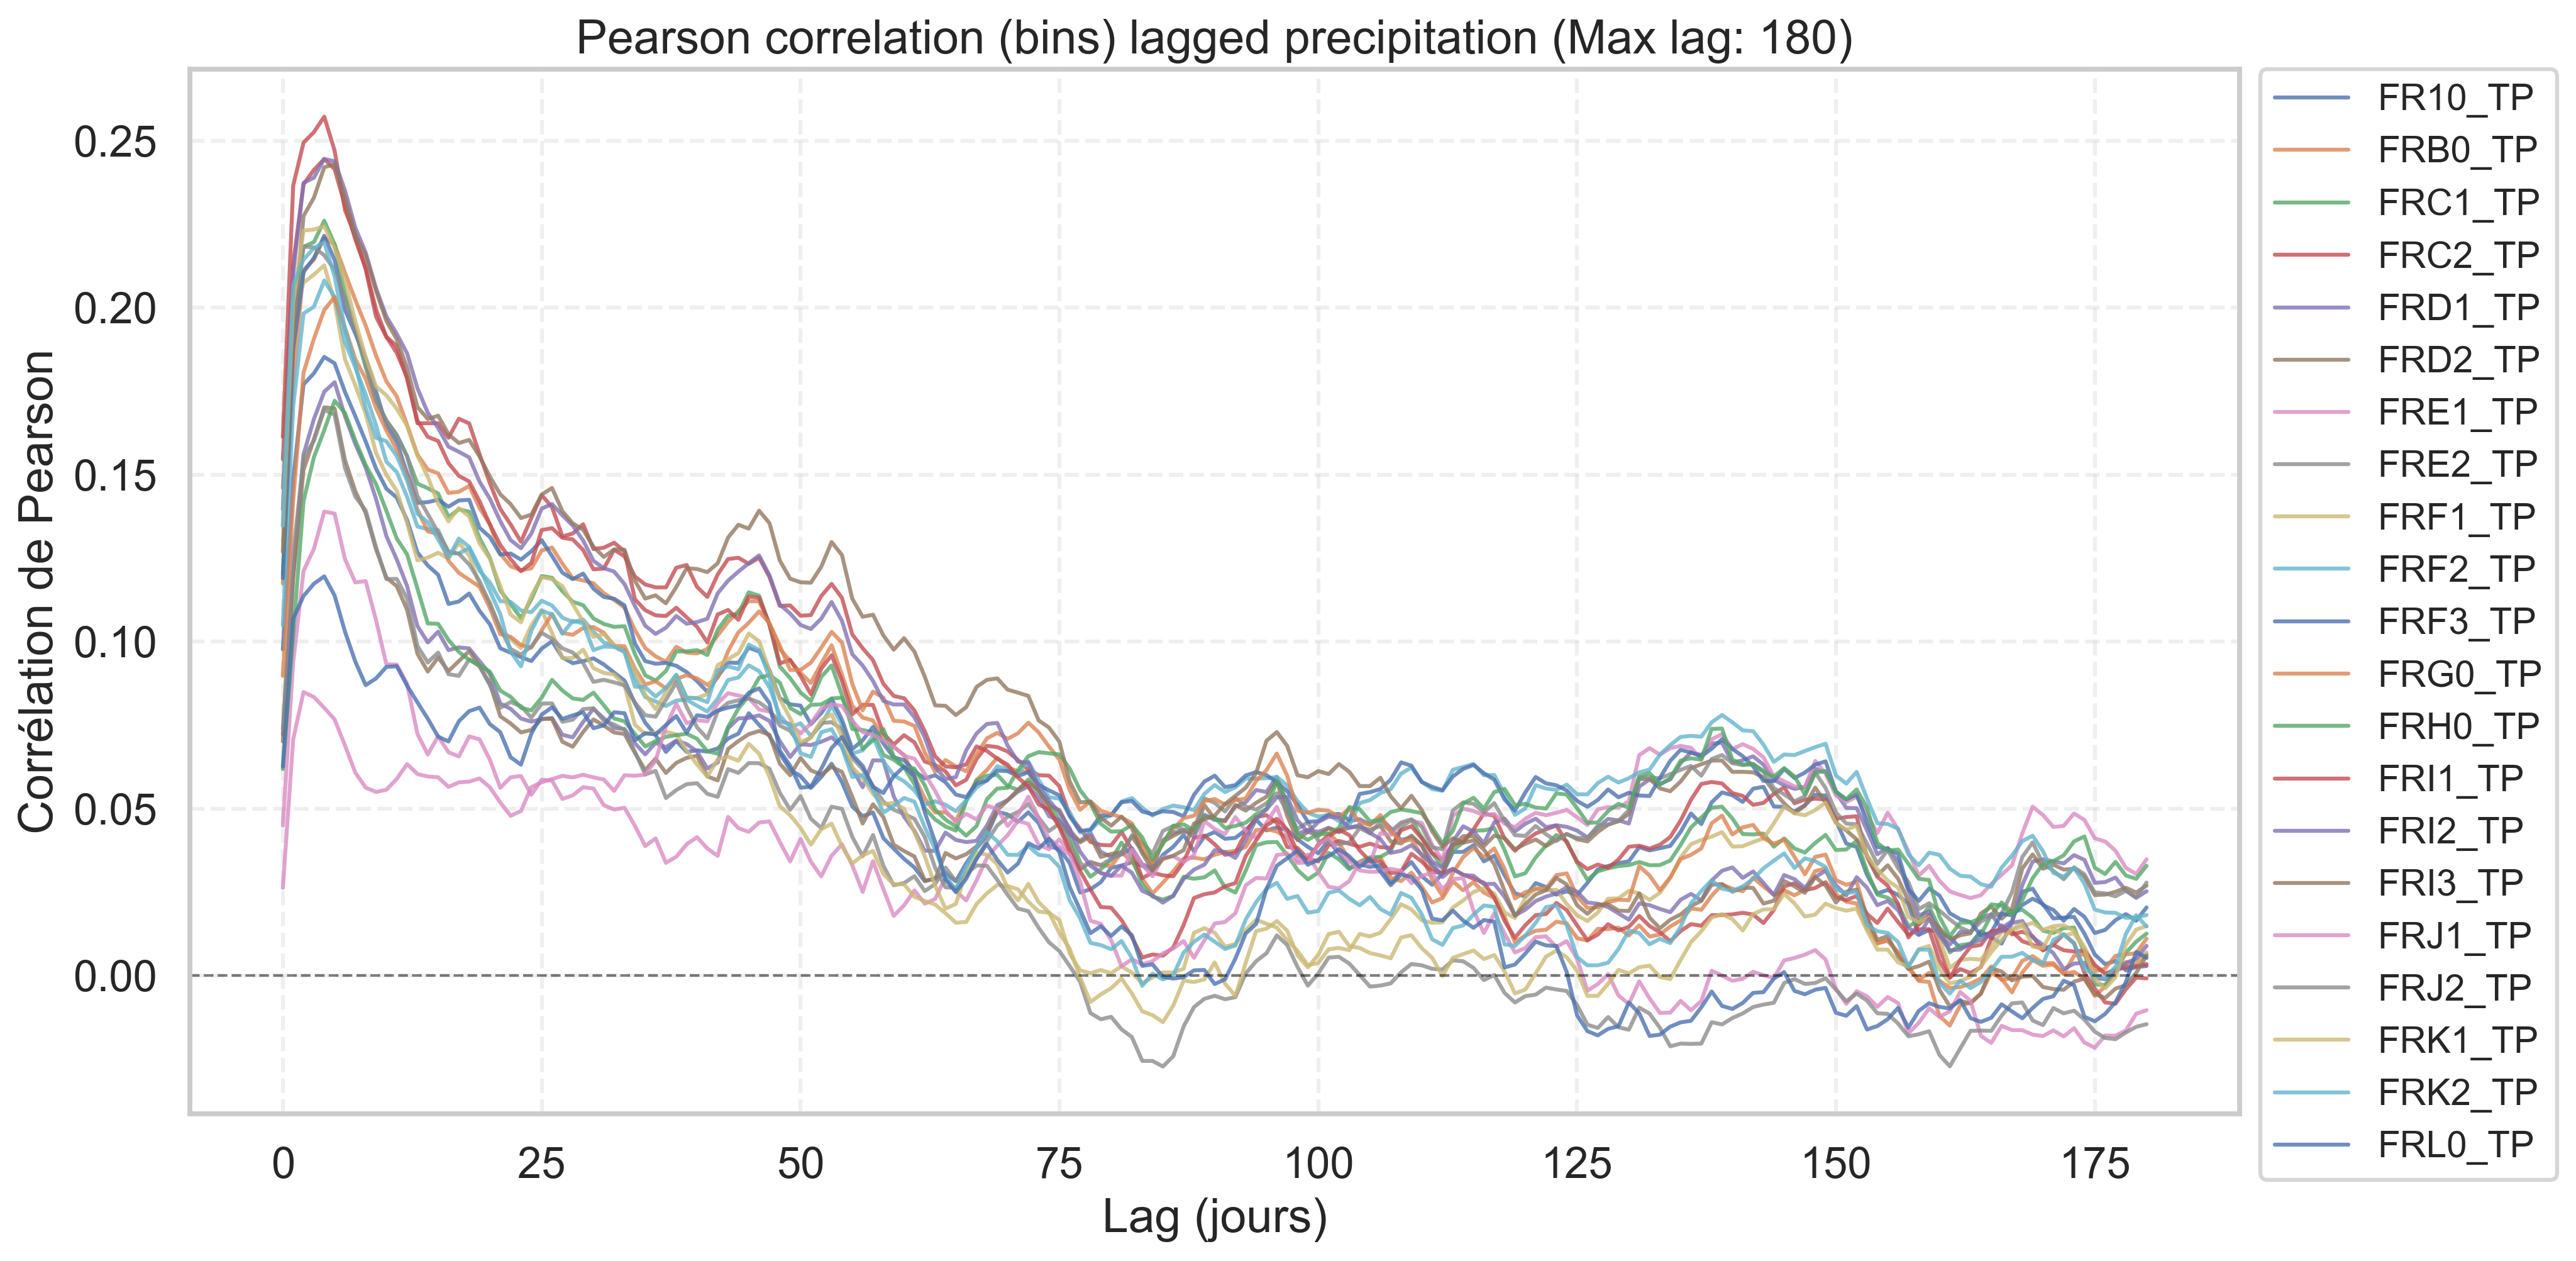
\includegraphics[width=\linewidth]{correlation_tp_lag.png}
  \caption{Optimisation des lags pour la précipitation}
\end{figure}


\begin{figure}[h!]
  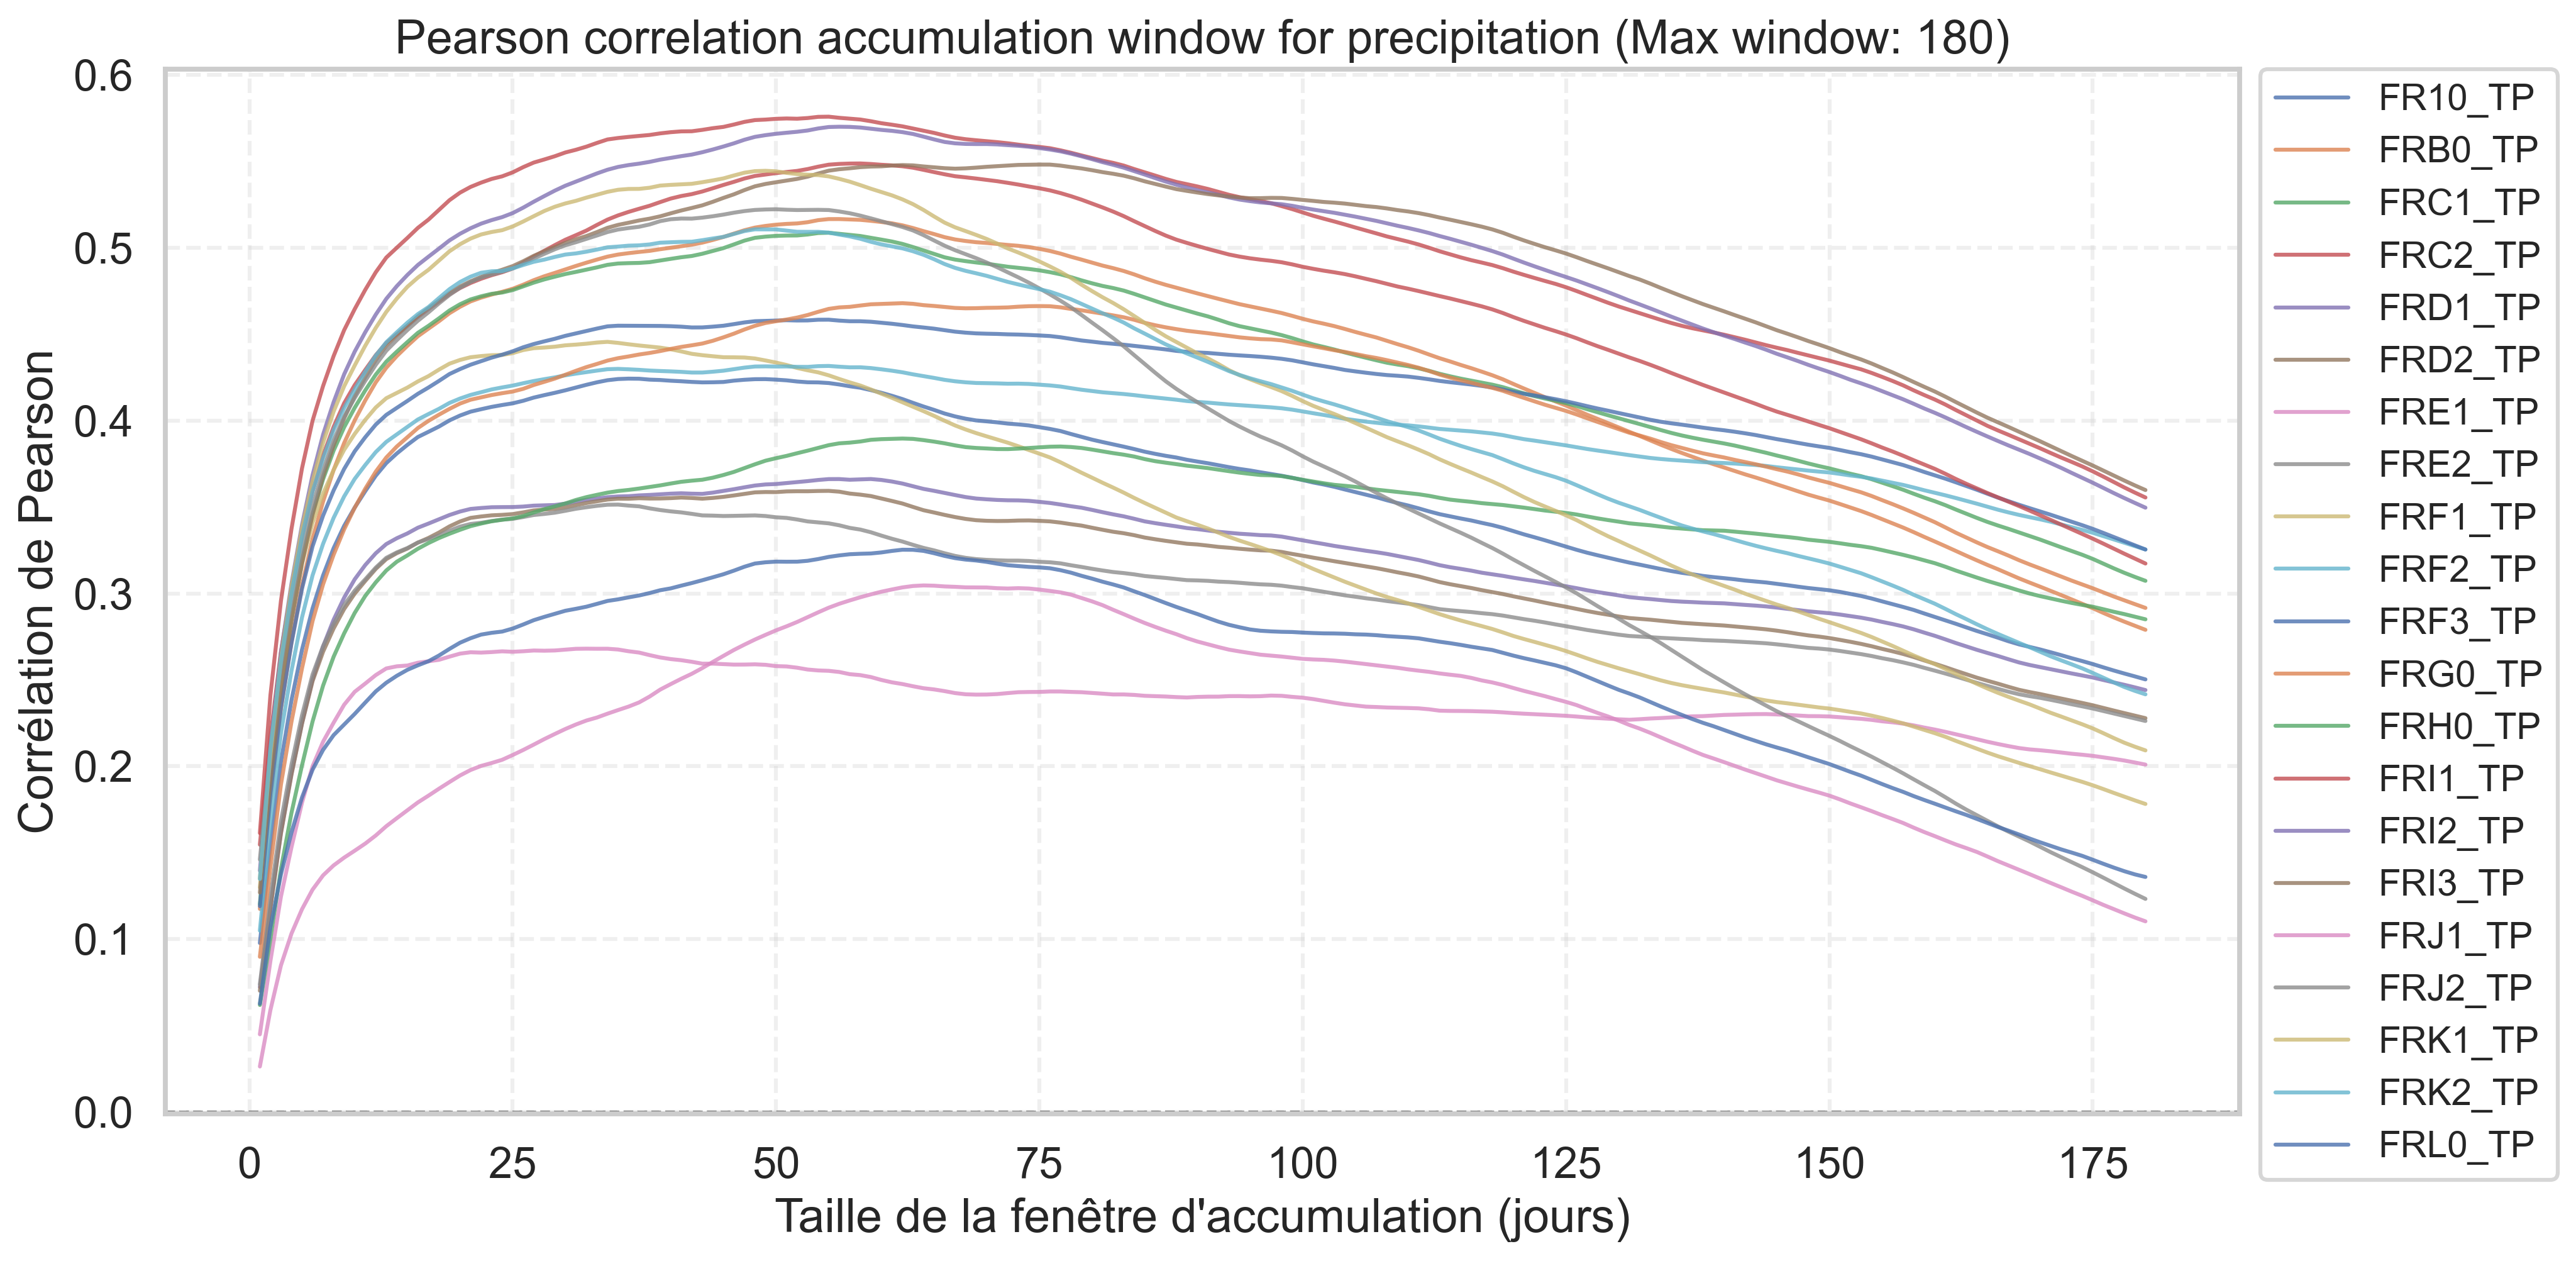
\includegraphics[width=\linewidth]{correlation_tp_accumulation_window.png}
  \caption{Optimisation des windows pour la précipitation}
\end{figure}

\subsection{Le fléau de la dimension}

L'augmentation naïve du nombre de features expose le modèle au risque de sur-apprentissage (\textit{overfitting}). Ce phénomène est une conséquence directe du \textit{fléau de la dimension} (Curse of Dimensionality).

Lorsque la dimension $d$ de l'espace des features augmente, les données deviennent éparses et la notion de distance euclidienne perd sa capacité discriminante.
Géométriquement, considérons l'hypercube unité $[0,1]^d$. La distance entre le centre et un sommet est $\frac{\sqrt{d}}{2}$, qui diverge quand $d \to +\infty$.
À l'inverse, le volume de l'hypersphère inscrite de rayon $R$ tend vers 0. Le volume $V_d(R)$ est donné par :
\[ V_d(R) = \frac{\pi^{d/2}}{\Gamma(\frac{d}{2} + 1)} R^d \]
où $\Gamma$ est la fonction Gamma d'Euler ($\Gamma(n) = (n-1)!$).
Comme $\Gamma$ croît factoriellement au dénominateur, on a $\lim_{d \to +\infty} V_d(1) = 0$. Cela implique qu'en grande dimension, la quasi-totalité du volume de l'hypercube se concentre dans ses "coins". Il faudrait alors un très (très) grand nombre de données d'apprentissage pour recouvrir l'espace de façon significative. Dans notre étude, le nombre de données d'apprentissage est assez limité (environ 5000).

\subsection{Stratégies de réduction de dimension}

Pour pallier ce problème, deux approches ont été considérées.

\subsubsection*{Analyse en Composantes Principales (ACP)}
L'ACP est une méthode mathématique de réduction de dimension par projection orthogonale. Elle consiste à déterminer les axes de plus grande variance des données.
Soit $\mathbf{X}$ la matrice des données centrées-réduites et $\Sigma = \frac{1}{n}\mathbf{X}^T\mathbf{X}$ la matrice de covariance.
D'après le théorème spectral, $\Sigma$ étant symétrique réelle, elle est diagonalisable dans une base orthonormée :
\[ \Sigma = P \Lambda P^T \]
Les vecteurs propres (colonnes de $P$) associés aux plus grandes valeurs propres (éléments de $\Lambda$) forment les nouvelles features (composantes principales). Bien qu'optimale pour conserver l'information statistique, l'ACP produit des variables qui sont des combinaisons linéaires de toutes les entrées, nuisant à l'interprétabilité physique.

\subsubsection*{Sélection par connaissance métier (Approche retenue)}
Nous avons privilégié une réduction de dimension basée sur la physique du problème pour conserver l'explicabilité du modèle.
Nous avons opéré une sélection spatiale :
\begin{enumerate}
    \item Agrégation par moyennes pondérées nationales sur certaines variables.
    \item Filtrage régional sélectif : nous ne conservons que les régions ayant un impact hydrologique majeur sur le CF national. Par exemple, les données de la région PACA (riche en centrales au fil de l'eau et reliefs) sont conservées, tandis que celles du Nord (faible relief, faible contribution au mix hydroélectrique) sont écartées.
\end{enumerate}

\newpage
\section{Machine Learning}
\subsection{Approche Linéaire }

L'approche linéaire consiste à modéliser le système à l'aide de fonctions linéaires : c'est une approche assez simple à implémenter et à concevoir à l'aide de la descente de gradient, mais ce n'est pas la plus performante.  

La régression linéaire est l’un des modèles les plus simples, les plus anciens et les plus utilisés en \textit{Machine Learning}. Elle appartient à la famille des modèles supervisés et est principalement employée pour résoudre des problèmes de \textbf{régression}, c’est-à-dire des tâches dont l’objectif est de prédire une variable numérique continue. 

Le principe fondamental de la régression linéaire repose sur l’hypothèse qu’il existe une \textbf{relation linéaire} entre une ou plusieurs variables explicatives (ou variables indépendantes) et une variable cible (ou variable dépendante). Dans le cas le plus simple, cette relation peut s’écrire sous la forme suivante :
\[
y = ax + b
\]
où $x$ représente la variable explicative, $y$ la variable cible, $a$ le coefficient directeur de la droite et $b$ l’ordonnée à l’origine.

\\
De manière plus précise, si la dimension est $n > 1$. Soit $S = \{(\mathbf{x}_1, y_1), \dots, (\mathbf{x}_N, y_N)\}$ l'ensemble d'apprentissage avec $\mathbf{x}_i \in \mathbb{R}^d$ et $y_i \in \mathbb{R}$.
\\

Choisissons la fonction hypothèse comme une fonction affine des caractéristiques d'entrée :
$$h(\mathbf{x}; \mathbf{w}) = w_0 + \mathbf{w}^T \mathbf{x} = w_0 + \sum_{i=1}^{d} w_i x_i.$$

Par abus de notation, on peut définir
$$\mathbf{x} = \begin{bmatrix}
1 \\
x_1 \\
\vdots \\
x_d
\end{bmatrix}, \quad \mathbf{w} = \begin{bmatrix}
w_0 \\
w_1 \\
\vdots \\
w_d
\end{bmatrix}$$

de sorte que
$$h(\mathbf{x}; \mathbf{w}) = \mathbf{w}^T \mathbf{x} = \sum_{i=0}^{d} w_i x_i.$$
\\

Ainsi, l’objectif principal de la régression linéaire est de déterminer les paramètres du modèle (les coefficients $w_i$ et le biais $b$) de manière à minimiser l’erreur entre les valeurs prédites par le modèle et les valeurs réelles observées dans les données. Cette optimisation est généralement réalisée à l’aide de la \textbf{méthode des moindres carrés}, qui consiste à minimiser la somme des carrés des erreurs. \\


Ici, nous nous sommes concentrées sur le modèle Ridge ou \textit{régularisation}. C'est une technique souvent utilisée pour contrôler le phénomène de sur-apprentissage (overfitting). \\
On ajoute un terme de pénalité qui décourage les coefficients de prendre des valeurs trop grandes.

$$\mathbf{w}^* = \operatorname{argmin}_{\mathbf{w}} E(\mathbf{w}) =: \frac{1}{2} \sum_{i=1}^{N} (w_0 + \mathbf{w}^T \mathbf{x}_i - y_i)^2 + \frac{\lambda}{2} \sum_{j=1}^{d} w_j^2$$

où $\lambda \geq 0$ est le paramètre de pénalité de complexité. Cette technique est également appelée \textit{weight decay}.

\subsubsection*{Remarques :}

\begin{itemize}
    \item[$\blacktriangleright$] Il n'y a pas de régularisation sur $w_0$
    \item[$\blacktriangleright$] $\sum_{i=1}^{d} w_i^2 = \mathbf{w}^T \mathbf{w} = \|\mathbf{w}\|_2^2$
    \item[$\blacktriangleright$] $\mathbf{w}^* = (X^T X + \lambda I_d)^{-1} X^T \mathbf{y}$
\end{itemize}

Ainsi, après mise en oeuvre puis optimisation du modèle, nous avons obtenu les résultats suivant : 

 \begin{figure} [H]

\centrage


\includegraphics[width=0.6\textwidth]{CF predictions.png}

\caption{Prédiction des facteurs de charge sur l'année 2023}

\étiquette{fig:CF 2023}
s
\end{figure} 

\begin{figure} [H]

\centrage

\includegraphics[width=0.6\textwidth]{actuel vs predicted.png}

\caption{Comparaison prédiction et réalité}

\étiquette{fig:actuel vs predicted}

\end{figure} 



Et, si ces résultats ne sont pas exploitables, ils montrent néanmoins qu'il est possible d'améliorer significatviement la performance d'un modèle. 
Cependant, du fait de sa simplicité, la régression linéaire présente certaines limites. En effet, elle suppose une relation linéaire entre les variables, ce qui n’est pas toujours le cas dans des situations réelles plus complexes. Elle peut donc manquer de précision lorsque les données présentent des interactions non linéaires ou des structures plus élaborées.

\newpage

\section{Les arbres de décision}

Face aux limites des modèles linéaires, il est parfois nécessaire de recourir à des méthodes plus flexibles et plus puissantes, comme les \textbf{arbres de décision}. Ces derniers sont des modèles de \textit{Machine Learning} capables de s’adapter à des relations complexes entre les variables.

Les arbres de décision peuvent être utilisés aussi bien pour des tâches de \textbf{classification}, où l’objectif est de prédire une catégorie ou une classe, que pour des tâches de \textbf{régression}, où l’on cherche à prédire une valeur numérique continue.

La caractéristique la plus distinctive des arbres de décision est leur \textbf{structure arborescente}, qui contribue fortement à leur simplicité de compréhension et à leur grande interprétabilité. Un arbre de décision est composé de plusieurs éléments essentiels :

\begin{itemize}
    \item \textbf{La racine} : il s’agit du premier nœud situé en haut de l’arbre. Elle représente l’ensemble complet des données d’apprentissage et correspond au premier test effectué sur les données.
    
    \item \textbf{Les nœuds internes} : ces nœuds effectuent des tests conditionnels simples sur une variable explicative (par exemple, $x < c$). Chaque test divise l’espace des données en sous-ensembles, créant ainsi une partition binaire de l’espace des variables d’entrée.
    
    \item \textbf{Les nœuds terminaux}, également appelés \textbf{feuilles} : situés en bas de l’arbre, ils correspondent aux décisions finales du modèle. Dans le cas d’un arbre de régression, la valeur prédite dans une feuille est généralement la moyenne des valeurs de la variable cible associées aux observations présentes dans cette région.
\end{itemize}

De manière conventionnelle, les arbres de décision sont représentés à l’envers, avec la racine en haut et les feuilles en bas. Cette représentation visuelle illustre clairement la succession de décisions prises par le modèle, depuis l’ensemble global des données jusqu’à la prédiction finale.

Grâce à leur structure intuitive, les arbres de décision sont particulièrement appréciés pour leur capacité à être interprétés facilement, contrairement à certains modèles plus complexes comme les réseaux de neurones. Toutefois, ils peuvent être sensibles au sur-apprentissage, ce qui nécessite souvent l’utilisation de techniques de régularisation ou de méthodes d’ensemble telles que les forêts aléatoires.




En mettant en place les différentes stratégies, nous avons pu obtenir : \\


[GRAPHIQUES ET COMMENTAIRES] \\



\subsection{Random Forest}
\label{subsec:rf}

Les \textbf{forêts aléatoires} (\textit{Random Forest}) constituent une méthode d'\textbf{ensemble} basée sur des \textbf{arbres de régression}. L’objectif est d’obtenir un modèle plus \textbf{robuste} qu’un arbre seul : en pratique, un arbre de décision peut très bien s’ajuster aux données d’entraînement mais il est souvent \textbf{instable} (forte variance). L’idée de Random Forest est donc de construire \emph{beaucoup} d’arbres volontairement variés, puis d’agréger leurs prédictions.

\subsubsection{Principe général : moyenne de plusieurs arbres}
On entraîne $B$ arbres de régression $\{\hat f_b\}_{b=1}^B$ et, pour une entrée $\mathbf{x}$, la prédiction finale est simplement la \textbf{moyenne} :
\[
\hat f_{\text{RF}}(\mathbf{x})=\frac{1}{B}\sum_{b=1}^{B}\hat f_b(\mathbf{x}).
\]
Cette moyenne réduit fortement la variance : même si chaque arbre est imparfait, leur combinaison tend à lisser les erreurs et à améliorer la généralisation.

\subsubsection{Pourquoi les arbres doivent être différents ? (décorrélation)}
Si tous les arbres se ressemblent, les erreurs se ressemblent aussi, et la moyenne apporte peu. Random Forest introduit donc deux sources d’aléa pour construire des arbres \textbf{décorrélés} :

\paragraph{1) Bagging (bootstrap)}
Chaque arbre est entraîné sur un \textbf{échantillon bootstrap} du jeu de données (tirage avec remise). Cela signifie que deux arbres ne voient pas exactement les mêmes observations, ce qui change leurs découpes et leurs feuilles.

\paragraph{2) Sous-ensemble aléatoire de variables à chaque split}
À chaque nœud d’un arbre, au lieu de tester toutes les variables, l’algorithme ne considère qu’un \textbf{sous-ensemble aléatoire} de variables (hyperparamètre \texttt{max\_features}). Ainsi, même si une variable est très prédictive, elle n’est pas systématiquement utilisée en premier, ce qui force les arbres à explorer des structures différentes.

\subsubsection{Estimation interne de l’erreur : \textit{Out-Of-Bag} (OOB)}
Avec le bootstrap, environ un tiers des observations ne sont \textbf{pas} utilisées pour entraîner un arbre donné : ce sont les données \textit{out-of-bag} pour cet arbre. On peut donc estimer la performance sans jeu de validation dédié :
pour chaque observation, on agrège uniquement les prédictions des arbres qui ne l’ont pas vue à l’entraînement, puis on calcule une erreur (MSE, MAE, $R^2$). Cette estimation OOB est très pratique pour comparer des réglages d’hyperparamètres.

\subsubsection{Hyperparamètres principaux}
Les paramètres les plus importants sont :
\begin{itemize}
    \item \texttt{n\_estimators} ($B$) : nombre d’arbres. Plus $B$ est grand, plus la prédiction se stabilise (au prix d’un coût de calcul supérieur).
    \item \texttt{max\_features} : nombre de variables candidates à chaque split. Plus il est petit, plus les arbres sont décorrélés (mais un réglage trop faible peut dégrader la précision).
    \item \texttt{max\_depth}, \texttt{min\_samples\_leaf} : contrôlent la complexité de chaque arbre et limitent le sur-apprentissage.
\end{itemize}

\subsubsection{Intérêt pour notre problème}
Dans notre cas, la relation entre variables climatiques (températures, précipitations, effets retardés via lags, saisonnalité) et facteur de charge est \textbf{non-linéaire} et comporte des \textbf{interactions}. Une Random Forest capture naturellement ces non-linéarités, tout en restant plus stable qu’un arbre unique. Elle offre aussi des outils d’analyse comme l’\textbf{importance des variables} (quelles entrées contribuent le plus à la prédiction du CF). \\

[RESULTATS RANDOM FOREST]\\

1. Sélection des variables et modélisation initiale \\
Dans un premier temps, afin de constituer un jeu de données optimisé, une étude de corrélation a été menée pour identifier les régions ayant l'influence la plus significative sur le facteur de charge. Sur la base de ces données, nous avons implémenté une première association de modèles de type Random Forest (via la librairie Scikit-learn) avec les hyperparamètres par défaut.\\
Les résultats obtenus sur les données brutes s'étant révélés insuffisants, une procédure d'optimisation par GridSearch a été appliquée. Bien que cette étape ait amélioré la précision globale, l'analyse des résidus a mis en évidence des motifs récurrents : les prédictions présentaient systématiquement une surestimation ou une sous-estimation par rapport aux données réelles.\\

2. Caractérisation du biais systématique \\
L'observation de ces écarts a suggéré l'existence d'un biais qu'il semblait possible de corriger linéairement. L'objectif a donc été de déterminer un « biais optimal » pour une année quelconque (ex: 2024, 2030). Pour ce faire, nous avons d'abord calculé le biais optimal rétrospectif pour chaque année de la période d'entraînement (2016-2022) en comparant les valeurs prédites aux valeurs réelles (voir code en annexe).\\

3. Développement d'un modèle hybride \\
Une première approche naïve, consistant à appliquer à l'année test (2023) la moyenne des biais des années précédentes, n'a pas produit de résultats concluants, contrairement à ce qui avait été observé avec la régression linéaire simple. La complexité du modèle Random Forest nécessitait une méthode de correction plus dynamique. \\
Nous avons par conséquent élaboré une architecture hybride. Celle-ci intègre un modèle secondaire de régression linéaire, entraîné sur les biais optimaux historiques (8 points de données) ainsi que sur les variables météorologiques (températures et précipitations). Ainsi, pour une année donnée, ce modèle secondaire prédit le biais correctif à appliquer en fonction des conditions climatiques. \\

4. Résultats et limites \\
L'intégration de cette correction a permis d'améliorer significativement les performances du modèle. Toutefois, une surestimation persiste sur l'année 2023. Cette limitation est principalement attribuable à la faible taille de l'échantillon utilisé pour l'entraînement du modèle correctif (seulement 8 années d'historique). Une perspective d'amélioration consisterait à étendre la plage temporelle des données d'entraînement aux années antérieures à 2015, afin d'accroître la robustesse statistique de la correction de biais. \\

[AUTRES RESULTATS ?]

\subsection{Gradient Boosting}
Le Gradient Boosting est également une technique utilisant les arbres et la récursion. Néanmoins, contrairement au Random Forest qui construit ses arbres en parallèle et de manière indépendante, le Gradient Boosting construit ses arbres de manière séquentielle et additive.Chacunde ces arbres peut être relativement petit et, en général, cela améliorer progressivement la précision du modèle. \\

Ensuite, nous avons cherché à développer un nouveau modèle de Machine Learning, s'appuyant sur l'algorithme de Gradient Boosting (ou XGBoost) pour améliorer encore plus nos prédictions. \\
L'algorithme de Gradient Boosting utilise lui aussi des arbres de décision et un principe itératif. Cependant, contrairement à l'algorithme de Random Forest, qui va construire parallèlement et de manière indépendante et aléatoire des arbres faibles de décision, cette nouvelle approche procède à cette construction de façon séquentielle et perturbative. L'objectif étant toujours le même : on va augmenter le nombre d'arbres, et réduire leur taille afin de mettre en commun leurs résultats et d'éviter le phénomène de sur-apprentissage et la dépendance envers le set d'entrainement. \\
Ainsi, le principe de cette méthode est le suivant : on vient ajuster la prédiction des arbres de décision sur les résidus du modèle précédent (et non la réponse), prédiction que l'on ajoute ensuite au modèle pour aboutir à une fonction ajustée plus précise sur les erreurs des modèles précédents. \\
En pratique, on commence par initialiser les valeurs cibles par les cibles $\{ y_{i} \}$ de l'ensemble d'entrainement. \\ 
On construit dans un premier temps un premier arbre de décision qui fournit une première approximation de la valeur cible avec une fonction $f_{1}$. \\
Le deuxième arbre que l'on construit va lui chercher à prédire les valeurs $y_{i} - f_{1}(x_{i})$ pour améliorer la prédiction du modèle, avec une fonction $f_{2}$. \\
Et ainsi de suite de façon récursive, à chaque étape, on perturbe les résidus de la prédiction qui vient d'être réalisée $$r_{i} \longleftarrow r_{i} + \lambda f_{i}(x_{i})$$ 
Le paramètre $\lambda$ correspond au taux d'apprentissage du modèle. \\

A la fin, au bout de $M$ itérations, la valeur qui est renvoyée correspond à la somme de toutes les prédictions :  $$f(x) = \sum_{i = 1}^{M}\lambda f_{i}(x)$$
Remarques :
\begin{itemize} 
    \item les arbres sont volontairement petits, avec un petit nombre de nœuds
    \item le taux d'apprentissage est lui aussi volontairement réduit
    \item Cela permet au modèle d'apprendre lentement et de limiter le sur-apprentissage en apprenant à préciser ses erreurs. 
    \item Le nombre d'arbres, leur profondeur, le nombre de nœuds, le taux d'apprentissage,... sont autant d'hyper-paramètres à optimiser par validation croisée lors du développement du modèle. 
\end{itemize}

[GRAPHIQUES ET COMMENTAIRES DES RESULTATS]


\newpage
\section{Deep Learning}

Nous nous sommes ensuite penchés sur une approche différente : le Deep Learning. C’est un autre sous-domaine de l'apprentissage automatique qui utilise des réseaux de neurones artificiels composés de nombreuses couches pour analyser des données et prendre des décisions.

En particulier, nous avons utilisé le modèle LSTM (Long Short-Term Memory, soit Mémoire à Long Terme et à Court Terme), qui est un type de réseau de neurones récurrents (RNN) particulièrement adapté pour traiter et prédire les séries temporelles et les séquences de données.\\


Le Deep learning étant un domaine large, nous avons choisi de nous concentrer sur le modèle LSTM pour \textit{Long Short Term Memory}. Cette architecture permet au Réseau Neuronal Récurrent de condeerver plus facilement les informations sur plusieurs étapes temporelles récurrentes. 

Les LSTM ne garantissent pas l’absence de problèmes de gradient
disparaissant/explosif, mais elles offrent au modèle un moyen plus simple d’apprendre les dépendances à longue distance.\\

\subsection{Introduction aux Réseaux de Neurones}

[EXPLIQUER LE PRINCIPE DE BASE ET LES RESULTATS OBTENUS]

\subsection{Réseaux de Neurones Récurrents pour Séries Temporelles}
Nous nous sommes ensuite penchés sur une approche différente et plus complexe : le Deep Learning. C'est un autre sous-domaine de l'apprentissage automatique qui utilise des réseaux de neurones artificiels composés de nombreuses couches pour analyser des données et prendre des décisions. 

\paragraph{Choix d'architecture pour des séries temporelles} \\
Les réseaux de neurones \emph{feedforward} (par exemple les MLP) constituent une première approche efficace pour l'apprentissage supervisé, mais présentent une limitation structurelle lorsqu'ils sont appliqués à des \textbf{séries temporelles} : ils ne modélisent pas explicitement la \textbf{dépendance séquentielle}. En pratique, un MLP traite chaque observation comme un vecteur ``statique'' et, sauf ingénierie de variables spécifique (retards, agrégations, encodage positionnel), il n'intègre pas naturellement le fait que l'ordre des mesures porte de l'information. Cette absence de mémoire interne rend l'extraction de dynamiques temporelles (inertie, effets retardés, saisonnalités et interactions dans le temps) plus difficile et souvent dépendante du choix de la fenêtre et des \emph{features} construites.

\paragraph{Réseaux récurrents et état caché} \\
Pour représenter cette dimension temporelle, nous avons retenu une architecture \textbf{récurrente} (\emph{Recurrent Neural Network}, RNN). Contrairement à une approche strictement instantanée, un RNN maintient un \textbf{état caché} $h_t$ mis à jour à chaque pas de temps : la prédiction à l'instant $t$ dépend à la fois de l'entrée courante $x_t$ et du contexte accumulé via $h_{t-1}$. Ce mécanisme confère au modèle une forme de mémoire, permettant d'exploiter des dépendances de court terme sans imposer explicitement une représentation \emph{ad hoc} des retards.

\paragraph{LSTM et problème de disparition du gradient} \\
Nous avons plus spécifiquement implémenté un \textbf{LSTM} (\emph{Long Short-Term Memory}), conçu pour atténuer une difficulté majeure des RNN standards : la \textbf{disparition du gradient} (\emph{vanishing gradient}), qui limite l'apprentissage de dépendances à long terme lors de la rétropropagation à travers de longues séquences. Le LSTM introduit une \textbf{mémoire interne} (souvent notée $c_t$) et un système de \textbf{portes} (\emph{gates}) qui contrôlent le flux d'information :
\begin{itemize}
    \item une \emph{porte d'oubli} régule la conservation ou la suppression d'informations passées ;
    \item une \emph{porte d'entrée} contrôle l'intégration de nouvelles informations ;
    \item une \emph{porte de sortie} détermine la part de mémoire exposée à la couche suivante.
\end{itemize}
En régulant ces opérations, le LSTM stabilise l'apprentissage et permet de capturer des motifs temporels plus persistants que ceux généralement accessibles à un RNN simple.

\paragraph{Stacked LSTM et apprentissage hiérarchique} \\
Afin d'augmenter la capacité de représentation, nous avons utilisé un \textbf{Stacked LSTM} (LSTM empilé), c'est-à-dire une architecture où plusieurs couches LSTM sont superposées. La sortie de la première couche sert d'entrée à la seconde, et ainsi de suite. Cette profondeur permet d'apprendre une hiérarchie de représentations : les couches inférieures tendent à capter des régularités locales (variations rapides, corrélations de court terme), tandis que les couches supérieures peuvent modéliser des structures plus \textbf{abstraites} et \textbf{non linéaires} (tendances, interactions complexes entre variables, dépendances plus longues).

\paragraph{Résultats et limites de généralisation} \\
Dans notre cas, les performances obtenues sur l'année \textbf{2023} se sont révélées très élevées, malgré un ensemble de variables explicatives limité : les entrées sont principalement des \textbf{moyennes nationales}, construites à partir de fenêtres temporelles différentes pour les \textbf{précipitations} et les \textbf{températures}. Une première analyse a toutefois mis en évidence un biais méthodologique : l'absence initiale de \textbf{jeu de validation}. Sans séparation temporelle stricte, le modèle peut s'ajuster excessivement aux spécificités de 2023 (surapprentissage), ce qui conduit à des résultats flatteurs en apparence, mais à une \textbf{faible capacité de généralisation}. \\
[METTRE LES GRAPHIQUES]



\paragraph{Synthèse} \\
En synthèse, le choix d'un \textbf{(Stacked) LSTM} répond à l'enjeu de modélisation séquentielle et au problème de \emph{vanishing gradient} grâce aux mécanismes de portes. Toutefois, ces résultats soulignent que de bonnes performances \emph{in-sample} (ou sur une période proche) ne garantissent pas la robustesse en projection lointaine ; une validation temporelle stricte et des tests de généralisation hors distribution sont indispensables pour conclure à la fiabilité des prédictions à horizon 2050.
Nous avons ensuite corrigé ce point en introduisant un jeu de validation basé sur \textbf{2022} (découpage temporel). Les métriques sur 2023 restaient favorables, suggérant une bonne adéquation au régime de données observé. Néanmoins, une évaluation plus exigeante a montré une \textbf{résilience insuffisante} : lors d'une extrapolation vers des conditions projetées (par exemple \textbf{2050}), les prédictions produites n'étaient pas jugées recevables. Ce comportement indique que, malgré l'apport du LSTM pour apprendre des dépendances temporelles, le modèle demeure sensible aux \textbf{changements de distribution} (\emph{distribution shift}) et peut échouer hors du domaine couvert par les données d'entraînement (non-stationnarités climatiques, nouvelles amplitudes, nouvelles corrélations entre variables).

\newpage

\section{Résultats}
Les résultats obtenus selon les modèles sont les suivants : \\

\begin{table}[H]
    \centering
    \begin{tabular}{|c|c|c|c|c|} % Ajout des | pour les lignes verticales
    \hline % Ligne horizontale supérieure
    \textbf{Modèle} & \textbf{R}^2 & \textbf{nMAE} & \textbf{nRMSE} & \textbf{R} \\
    \hline % Ligne horizontale séparant les en-têtes des données
    Ridge Regression & 0.58&0.14 & 0.18& 0.76\\
    \hline
    Random Forest & 0.66 & 0.16 & 0.19 & 0.83\\
    \hline
    Gradient Boosting & 0.66 &0.13 & 0.17 &0.82\\
    \hline
    LSTM & 0.71 &0.11 & 0.15& 0.85\\
    \hline % Ligne horizontale inférieure
    \end{tabular}
    \caption{Tableau récapitulatif des meilleurs résultats par modèle} % Caption plus claire
    \label{tab:tableau_recapitulatif_resultats} % Label standardisé
\end{table}

En comparant toutes les différentes métriques d'erreurs, on remarque que le modèle LSTM est celui qui donne les meilleurs résultats, c'est pourquoi nous l'avons choisi pour la partie prospective. \\
Facteurs limitants de nos résultats: 
\begin{itemize}
    \item manque de données: nous n'avons accès qu'aux données de précipitation et température au niveau régional, ce qui est insuffisant pour prédire la facteur de charge. Les données d'ouvertures de barrages etc.. pourrait être plus pertinentes
    \item facteur humain: toute l'eau des pluies ne va pas dans les centrales hydroélectriques, il y a des pertes, des usages agricoles, touristiques etc.. comme nous l'avons vu lors de la visite de la centrale de Sainte Tule. En effet, le réglage du barrage sert aussi à maintenir un lac artificiel contenant des activtiés touristiques.
\end{itemize}

\newpage


\section{Prospective}

Après avoir mis en place différents modèles de Machine Learning et de Deep Learning pour prédire les facteurs de capacité des barrages hydroélectriques au fil de l'eau en France, nous avons utilisé le modèle le plus performant, à savoir le LSTM, pour réaliser une étude prospective, ce qui constitue l'objectif principal de ce projet. \\

A l'aide des données climatiques issues des scénarios RCP4.5 et RCP8.5, nous avons pu obtenir des prévisions de températures et de précipitations journalières en France à l'horizon 2050. En utilisant ces données comme entrées pour notre modèle LSTM, nous avons pu prédire les facteurs de capacité des barrages hydroélectriques au fil de l'eau en 2050. \\
Nous obtenons les courbes ci-dessous: \\


Critiques des résultats obtenus : \\
Si nous comparons avec les données de 2023 et 2022 en traçant l'enveloppe sur le même grapique, nous voyons que les variations ont quasiment disparus et que la moyenne est effectivement plus basse. \\
Le lissage des données climatiques sur 10 ans a eu pour effet de lisser les variations journalières, ce qui n'est pas réaliste. En effet, les barrages au fil de l'eau sont très sensibles aux variations climatiques journalières, et il est donc important de conserver ces variations pour obtenir des prévisions plus précises. \\
Une explication potentielle serait que les différence été hiver sont moindre car l'accumulation de neige en hiver est moins importante dans les scénarios climatiques futurs. Ce qui réduit la différence saisonnière. \\ 
Il est en revanche très complexe de justifier l'abscence du puit de la fin de l'été.

\subsection{Prévision contre Prospective}

Nous nous inscrivons ici dans une démarche de prospective. Aujourd'hui, elle correspond à une démarche de réflexion et d'anticipation autour de scénarios futurs pour notre société. Elle se met en place à travers une approche holistique : elle intègre un grand nombre de données et de paramètres, et ce afin de créer des scénarios qui pourraient coller le mieux avec notre réalité future, sans laisser de zones d'ombres, qui n'auront pas été traitées. \\

Il est important de souligner que la prospective se différencie de la prévision, malgré de nombreuses ressemblances de prime abord.

De fait, la prévision vise à des échelles de temps relativement courtes -de l'ordre de l'année-, et se concentre sur l'élaboration d'un unique scénario : une ligne directrice unique qui serait à suivre.\\

La prospective, quant à elle, vise à des horizons plus lointains (de l'ordre de la dizaine d'année), et s'inscrit dans l'exploration de nombreux scénarios. L'idée est ici de construire non pas un avenir, mais des avenirs, qui laisseraient la possibilité d'opérer à des changements majeurs dans certains secteurs donnés de notre société, selon l'évolution réelle qui se fera de cette dernière. Le but est donc d'explorer un grand nombre de scénarios afin d'avoir envisagé toutes les éventualités, et ainsi de ne pas être pris au dépourvu, lorsqu'il est nécessaire de fixer des directives dans des secteurs donnés (énergétique, économie, etc.).

\subsection{Le Modèle Times-France}

Le modèle Times-France est issu de la famille de modèles  MARKAL/TIMES (MARKet ALlocation/ The Integrated Markal Efom (Energy Flow Optimization Model) System). Cette famille de modèles est à la base du programme en modélisation prospective du Centre de Mathématiques Appliquées (CMA) des Mines de Paris. \\
Initialement, ces modèles se concentraient uniquement sur la gestion de l'électricité, mais ils se sont étendu à l'entiéreté du système énergétique. 
 Ils peuvent se déployer sur différentes échelles : la France, l'Europe, ou le monde. Par la suite, le CMA s'est concentré sur le développement d'un modèle spécifique à la France, qui évolue en permanence depuis 2003 afin de s'adapter le plus possible aux évolutions constantes du système énergétique français. C'est donc un modèle adaptable, qui est développé et amélioré en continu. \\
 Ces évolutions permanentes se font notamment autour de la modélisation de la biomasse, des secteurs électriques, résidentiels et des transports français. Il est en outre important de prendre en compte les mises à jour des bases de données technologiques, qui influent fortement sur la demande en énergie (par exemple les data centers : forte demande en électricté, apport en eau pour les circuits de refroidissement, etc.). En outre, des approfondissements récents ont été mis en place autour de la représentation de la flexibilité des systèmes qui se basent sur plusieurs sources énergétiques (intermittentes ou non), mais aussi sur l'influence de l'évolution des modes de vie et de consommation des ménages sur la demande en services énergétiques. \\

 Nous nous sommes basés sur le modèle Times-France, avec l'aide d'Edi ASSOUMOU (CMA MINES ParisTech) pour mettre en place notre démarche de prospective. \\
 Le modèle Times-France se base sur une représentation technico-économique du système énergétique français, et cherche à optimiser cette représentation en minimisant les coûts d'investissements réalisés dans ce secteur. Cela veut dire que pour un jeu de donnéess d'entrée fixé, le modèle nous donnera en sortie un mix énergétique pour la France à un horizon de temps que nous aurons fixé, qui correspond aux contraintes que nous aurons imposé, tout en minimisant les coûts d'investissements réalisés entre l'année de départ et l'année horizon dans le système énergétique, pour atteindre ce mix énergétique futur. En d'autres termes, nous avons en sortie le mix énergétique le moins cher, au sens propre du terme. \\

 C'est en outre un modèle linéaire. Il prend en entrée un grand nombre de données, parmi lesquelles :
 \begin{itemize}
 \item La capacité installée actuelle en France par source d'énergie
 \item La croissance de la consommation énergétique per capita estimée entre aujourd'hui et l'année horizon
 \item La population française estimée en 2050
 \item Le capacity credit attribué à chaque source en énergie : il permet de mesurer la fiabilité d'une centrale électrique. Il correspond à la fraction de la capacité installée d'une centrale électrique sur laquelle on peut compter avec certitude à un instant donné (typiquement lors d'un pic de demande). Il peut donc être fixé à 1 pour le nucléaire ou le thermique à flamme, mais il est bien plus faible pour les énergies renouvelables telles que l'éolien ou le solaire, qui sont intermittentes et dépendent fortement des conditions météorologiques.
 \item Le nombre de voitures individuelles en France estimés pour l'année horizon
 \item etc...
 \end{itemize}
\\

Il établit ensuite des relations linéaires entre ces différentes données, en essayant de retranscrire au mieux la chaîne de demande énergétique en France. Le logiciel fait de plus apparaître explicitement les différents acteurs qui interviennent sur cette chaîne : import et production d'énergie, acheminement sur le territoire français, consommateurs (particuliers et entreprises...). Anisi, on a un fonctionnement par ramification, avec la possibilité d'intervenir à différents niveaux dans cette chaîne de demande. De plus, on peut aussi influer sur les contraintes législatives ou bien qui relèvent plus de l'opinion publique : on peut fixer la taxe carbone, ou aussi mettre en place la sortie du nucléaire, etc.\\

Il a donc été nécessaire pour nous de réfléchir aux endroits où il est pertinent d'intervenir.
 \begin{itemize}
 \item Au niveau des données d'entrée : est-on optimiste vis-à-vis de la confiance que l'on accorde aux énergies renouvelables (intervenir sur les valeurs attribuées aux capacity credits) ? Est-ce que l'on considère que l'on va vers la sobriété (peu de croissance de la demande énergétique per capita) ?
 \item Au niveau des différents liens : il est possible de couper l'acheminement sur le territoire, l'import ou la production de certaines sources d'énergie. Permet-on l'usage du biogaz ? Et celui du charbon ?
 \item Au niveau des contraintes législatives : à combien fixe-t-on la taxe carbone ? La sortie du nucléaire est-elle envisageable ?
 \end{itemize}
 
Certains choix peuvent sembler plus pertinents que d'autres : de fait, aujourd'hui, 65\% de la production électrique française est assurée par le nucléaire. De même, un retour à un usage prépondérant du charbon semble peu probable du fait de l'amenuisement des ressources et de l'objectif français d'atteindre le net 0 en terme d'émissions de GES d'ici à 2050.


Néanmoins, il s’agit du but même de la prospective de mettre en place tous ces scénarios, afin d’envisager le plus de futurs possibles, et de ne pas être pris au dépourvu.

\subsection{Les scénarios mis en place}

[EXPLIQUER LES SCENARIOS REALISES, LES CONTRAINTES FIXEES, ETC]

Tableau récapitulatif des paramètres : 
\begin{center}
\begin{tabular}{|m{4cm}|m{4cm}|m{4cm}|}
   \hline
   Évolution des paramètres & Scénario optimiste & Scénario pessimiste \\
   \hline
   Population & 70 millions & 70 millions \\
   \hline
   Demande en électricité & Stagnation par rapport à 2023 &  +1\% par an \\
   \hline
   Taxe carbone & Laissée au standard actuel & Supprimée \\
   \hline
   Capacity credit & PV : 5\% ; Wind onshore : 15\%  ; Wind offshore : 40\% & PV : 0 ; Wind onshore : 5\% ; Wind offshore : 15\% \\
   \hline
   Biogaz & 50 TWh de capacité installée & 16 TWh de capacité installée\\
   \hline
\end{tabular}
\end{center}

\subsection{Résultats}

[METTRE LES GRAPHIQUES, COMMENTER, JUSTIFIER NOS RESULTATS]

\newpage
\section{Conclusion}
Pour résumer, nous avons donc mis en place différents modèles de Machine Learning et de Deep Learning 
pour prédire les facteurs de capacité des barrages hydroélectriques au fil de l'eau en France, 
à partir de données météorologiques régionales (températures et précipitations) et journalières. 
Après avoir comparé les performances de ces différents modèles, nous avons retenu le modèle LSTM 
pour réaliser une étude prospective à l'horizon 2050. Cette étude comprend 2 scénarios : 
un scénario optimiste et un scénario pessimiste, et a permis de calculer le mix énergétique 
électrique français optimal du point de vu financier en fonction des contraintes fixées.\\

    Néanmoins, plusieurs améliorations pourraient être apportées à notre travail. \\
    
    Tout d'abord, le modèle de prédiction des facteurs de capacité ne peut pas prendre en compte 
l'influence humaine sur le débit des rivières. En effet, les barrages hydroélectriques sont régulés
par des opérateurs humains qui ajustent les débits en fonction de divers facteurs.
Par exemple, on ouvre les barrages pour répondre au pics de demande électrique,
anticiper la fonte des glaces. Et, on les ferme pour maintenir des niveaux d'eau
suffisants pour l'agriculture, l'approvisionnement en eau potable ou des activités 
touristiques, comme nous l'avons vu lors de notre visite de la centrale de Sainte-Tulle, 
avec le lac de Serre-Ponçon.\\

    De plus, comme nous avons travaillé avec que deux données spatiales, il serait pertinent 
d'en inclure davantage. Par exemple, en prenant en compte le profil des bassins versants,
la couverture du sol, l'évapotranspiration, ou encore les données de débit des rivières.
Ces données permettraient de mieux saisir la complexité du cycle de l'eau et d'améliorer
la précision des prédictions. En outre, les données temporelles étant limitées à 9 ans,
l'ajout de données historiques plus anciennes pourrait renforcer la robustesse des modèles.\\

    Enfin, pour la partie prospective, puisque le modèle Times-France fonctionne majoritairement
sur des relations linéaires, l'étude présente des incertitudes. Ensuite, le choix 
des scénarios est arbitraire et peut fortement influencer les résultats obtenus. Il serait 
donc intéressant d'explorer une gamme plus large de scénarios, en variant davantage les 
sensibilités du modèle.\\

    Nonobstant ces limites n'invalident aucunement notre travail, qui est une étude pospective
et non une prévision absolue. L'objectif est d'anticiper les futurs possibles
et de préparer des stratégies adaptées pour la gestion du système énergétique français,
avec comme objectif la décarbonisation de l'économie.\\

    Notons enfin que ce projet s'est concentré sur les moyens de production électrique
classiques (hydroélectricité, nucléaire, éolien, solaire, thermique à flamme),
et n'a pas pris en compte, par exemple, l'avènement potentiel de la fusion nucléaire,
qui est actuellement porté par le projet ITER. Projet, localisé en France, 
à Saint-Paul-lez-Durance, que nous nous avons la chance de visiter ! \\

[INSERER PHOTO]

    Pour finir, ce MIG fût une grande aventure, exigéeante sur le plan théorique, 
puisque nous avons eu de nombreux cours sur les concepts mathématiques derrière 
le machine learning et deep learning, mais aussi exenrichissante sur le plan pratique,
car nous avons développé nos propres modèles. De surcroît, nous avons appris à travailler
ensemble à 13, en se répartissant les tâches, en communiquant efficacement.\\

    C'est pourquoi, nous souhaitons remercier très chaleureusement nos encadrants, Eddy [spap nom],
Damien Corral et valentina Sessa, mais aussi tous les intervenants et partenaires : RTE, ITER, CMA. 

[INSERER PHOTO]

\section{Bibliographie}
[COMPLETER BIBLIO]

\end{document}
